\section{Introducción}

\subsection{El lenguaje Gobstones}

Gobstones\cite{Gobstones} [hablar sobre gobstones]

\subsection{Editores Proyectivos}

El término Editor Proyectivo fue acuñado por Martin Fowler en el año 2005\cite{Fowler}, al intentar plantear un ambiente de desarrollo donde el programador pudiera expresar sus ideas en términos de conceptos en lugar de texto. Lo que vemos como texto pasaría entonces a constituir una representación editable del concepto al que hace referencia (y al cual Fowler llama \textit{representación abstracta}).

De esta manera, los conceptos del lenguaje son el dominio de los editores proyectivos, y decimos que un programa es una \textit{representación abstracta} construida utilizando dichos conceptos. Para modificar esta representación el programador interactúa con una interfaz de usuario, llamada \textit{representación editable}, sobre la cual la \textit{representación abstracta} se \textit{proyecta} en forma de texto\cite{voelter2014projectional}. 

\begin{wrapfigure}[10]{r}{0.5\textwidth}
  \begin{center}
    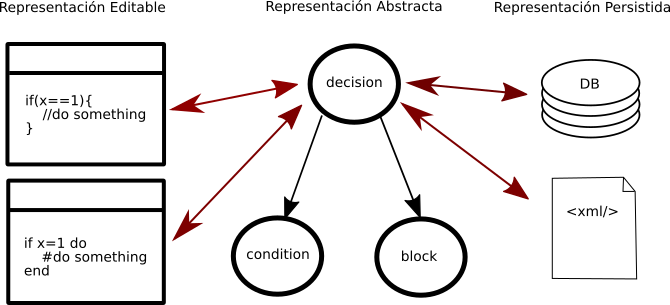
\includegraphics[width=0.5\textwidth,keepaspectratio]{assets/projectional-editor.png}
    \caption{Representaciones de un programa en un editor proyectivo}
  \end{center}
\end{wrapfigure}


A su vez, la \textit{representación abstracta} puede persistirse de diferentes maneras a diferentes soportes, con lo cual se introduce la idea de \textit{representación persistida} para hablar del formato en que guardará el programa, ya sea en una base de datos, un archivo binario, un texto con formato XML, etc.


Esto tiene varias consecuencias:
\begin{itemize}
  \item Deja de necesitarse un parser para el lenguaje, volviéndolo más sencillo de extender.
  \item El programador trabaja más cerca de los conceptos que quiere expresar.
  \item Deja de haber errores de sintaxis como tal.
  \item El editor trabaja directamente con las instancias de los conceptos, con lo cual:
  \begin{itemize}
    \item es más sencillo analizar el programa
    \item se simplifica la construcción de herramientas (ej: refactors, migrado de versiones de lenguaje, intentions, etc)
    \item se mejora la performance del editor al eliminarse la etapa de parseo.
  \end{itemize}
\end{itemize}



\subsection{MPS Workbench}



\cite{LanguageModularity}

\section{Problemática}

\section{Propuesta}

\section{Plan de trabajo}
